\begin{answer}
\newpage
Following is the printed output of the program. 
\begin{figure}[H]
  \centering
  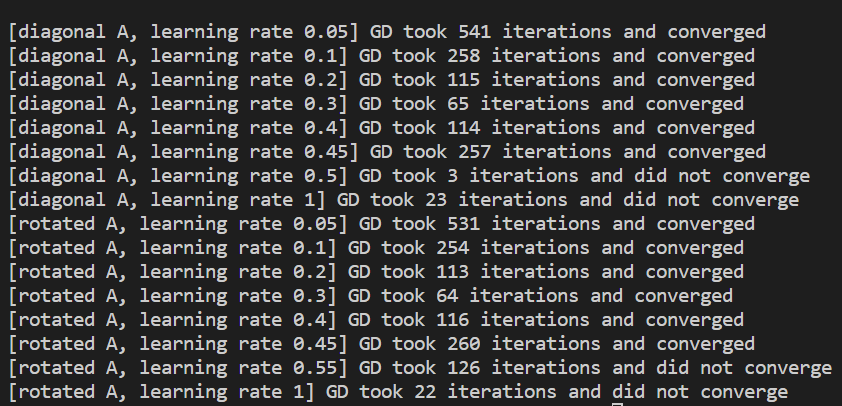
\includegraphics[width=0.9\textwidth]{gd_convergence/conv_rate_gd.PNG}
\end{figure}
We have that $\nabla J(\theta) = 2A\theta$, and therefore $\theta^{[t]} = (I-2\alpha A)^t\theta^{[0]}$. Thus by (b), GD converges if $0<\alpha<\frac{1}{A_{ii}}$, for all $i$.
From the output we see that GD converges for learning rate up until $\alpha = 0.5$, $max(A_{ii})=2$ so that matches the theoretical value. We also observe that the convergence is much slower for values close to the bounds, $(0, 0.5)$
\begin{figure}[H]
  \centering
  \begin{subfigure}[b]{0.49\textwidth}
    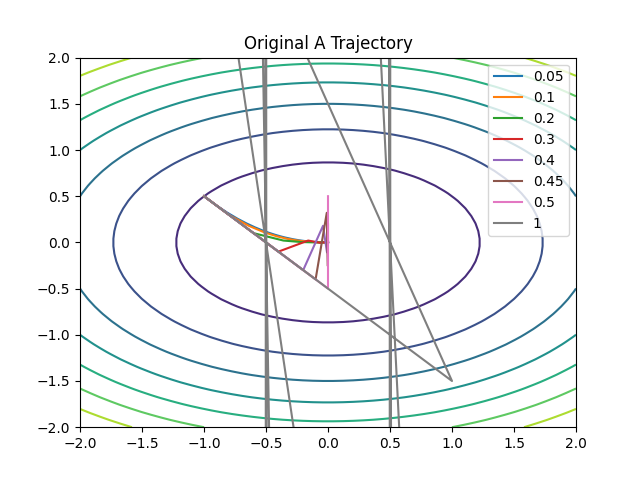
\includegraphics[width=\textwidth]{gd_convergence/trajectories.png}
  \end{subfigure}
  \begin{subfigure}[b]{0.49\textwidth}
    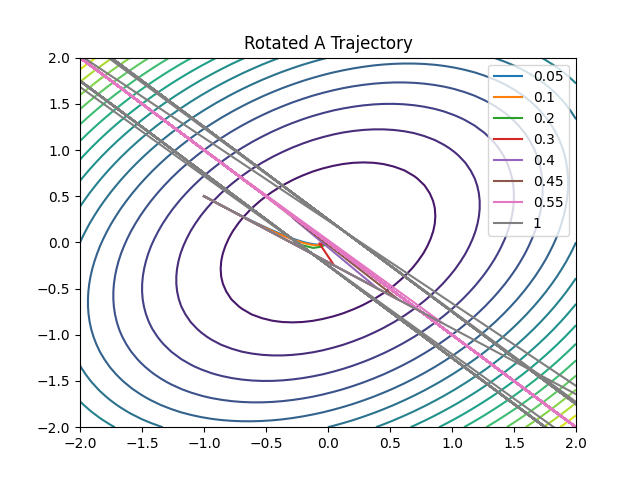
\includegraphics[width=\textwidth]{gd_convergence/trajectories_rotated.png}
  \end{subfigure}
\end{figure}
\newpage
\end{answer}